\documentclass[final]{beamer}
\usepackage[T1]{fontenc}
\usepackage[utf8]{inputenc}
\usepackage{lmodern}
\usepackage{amsmath,amssymb}
\usepackage{graphicx}
\usepackage{ragged2e}
\usepackage{array}
\usepackage{tikz}
\usepackage[size=custom,width=185,height=90,scale=1.70]{beamerposter}

\graphicspath{{./}{../figures/}}

\definecolor{FIMBlue}{RGB}{91,156,222}
\definecolor{FIMBlueDark}{RGB}{39,71,110}
\definecolor{FIMText}{RGB}{36,41,49}
\definecolor{FIMMuted}{RGB}{94,104,119}
\definecolor{FIMPanel}{RGB}{244,248,253}
\definecolor{FIMBorder}{RGB}{208,220,235}

\setbeamercolor{normal text}{fg=FIMText,bg=white}
\setbeamercolor{headline}{fg=white,bg=FIMBlueDark}
\setbeamercolor{block title}{fg=white,bg=FIMBlue}
\setbeamercolor{block body}{fg=FIMText,bg=white}
\setbeamercolor{itemize item}{fg=FIMText}
\setbeamercolor{itemize subitem}{fg=FIMText}

\setbeamerfont{title}{series=\bfseries,size=\fontsize{104}{112}}
\setbeamerfont{author}{size=\fontsize{40}{44}}
\setbeamerfont{institute}{size=\fontsize{30}{34}}
\setbeamerfont{block title}{series=\bfseries,size=\fontsize{44}{48}}
\setbeamerfont{block body}{size=\fontsize{31}{35}}
\setbeamerfont{caption}{size=\fontsize{22}{25}}

\setbeamertemplate{navigation symbols}{}
\setbeamertemplate{itemize item}{\raisebox{0.14em}{\tiny$\blacktriangleright$}}
\setbeamertemplate{itemize subitem}{\raisebox{0.14em}{\tiny$\blacktriangleright$}}
\setbeamertemplate{block begin}{%
  \vspace{0.18cm}
  \begin{center}
  \begin{beamercolorbox}[wd=0.965\linewidth,ht=1.42cm,dp=0.18cm,leftskip=0.38cm,rightskip=0.35cm]{block title}
    \usebeamerfont{block title}\strut\insertblocktitle\strut
  \end{beamercolorbox}
  \end{center}
  \vspace{0.16cm}
  \begin{beamercolorbox}[wd=\linewidth,sep=0.12cm]{block body}
    \usebeamerfont{block body}
}
\setbeamertemplate{block end}{%
  \end{beamercolorbox}
  \vspace{0.12cm}
}
\setlength{\leftmargini}{1.1em}
\setlength{\leftmarginii}{0.9em}
\setlength{\columnsep}{1.8cm}
\emergencystretch=3em

\pdfstringdefDisableCommands{%
  \def\textsuperscript#1{ (#1)}%
  \def\and{, }%
}

\hypersetup{
  pdftitle={Amortized In-Context Mixed Effect Transformer Models: A Zero-Shot Approach
for Pharmacokinetics},
  pdfauthor={Cesar Ojeda, Ramses J. Sanchez}
}

\title{Amortized In-Context Mixed Effect Transformer Models: A Zero-Shot Approach
for Pharmacokinetics}
\author{C\'esar Ojeda\textsuperscript{5} \and Rams\'es J. S\'anchez\textsuperscript{1,3} \and Wilhelm Huisinga\textsuperscript{5} \and Niklas Hartung\textsuperscript{5}}
\institute{\textsuperscript{1}Lamarr Institute \quad \textsuperscript{3}University of Bonn \quad \textsuperscript{5}University of Potsdam}

\newcommand{\FIM}{\textbf{FIM-PP}}
\newcommand{\FIMzs}{\textbf{FIM-PP} (zero-shot)}
\newcommand{\FIMft}{\textbf{FIM-PP} (fine-tuned)}
\newcommand{\dataset}[1]{\textbf{#1}}
\newcommand{\postersum}{\mathop{\raisebox{0.15ex}{\scalebox{4.0}[4.0]{$\displaystyle\sum$}}}\displaylimits}

\newcommand{\subhead}[1]{\vspace{0.25em}{\color{FIMText}\bfseries #1}\par\vspace{0.2em}}
\newcommand{\emline}[1]{{\color{FIMBlueDark}\bfseries #1}}
\newcommand{\logoimg}[1]{\includegraphics[height=6.1cm,keepaspectratio]{#1}}
\newcommand{\tightfigure}[3]{%
  \begin{figure}
    \centering
    \includegraphics[width=\linewidth,height=#2,keepaspectratio]{#1}
    \caption{#3}
  \end{figure}
}
\newcommand{\eqpanel}[1]{%
  \begin{beamercolorbox}[wd=\linewidth,rounded=true,sep=0.7em]{block body}
    #1
  \end{beamercolorbox}
}
\newcommand{\metricbox}[2]{%
  \begin{beamercolorbox}[wd=\linewidth,rounded=true,sep=0.85em]{block body}
    {\color{FIMBlueDark}\bfseries #1}\par
    \vspace{0.2em}
    #2
  \end{beamercolorbox}
}

\begin{document}
\begin{frame}[t]

\begin{beamercolorbox}[wd=\paperwidth,sep=1.35cm,leftskip=3.8cm,rightskip=2.0cm]{block body}
  \begin{columns}[T,totalwidth=\textwidth]
    \begin{column}{0.54\textwidth}
      \hspace*{0.9cm}\parbox[t]{0.94\linewidth}{%
        {\usebeamerfont{title}\color{FIMText}\inserttitle\par}
        \vspace{0.6cm}
        {\usebeamerfont{author}\color{FIMText}\insertauthor\par}
        \vspace{0.25cm}
        {\usebeamerfont{institute}\color{FIMMuted}\insertinstitute\par}
        \vspace{0.25cm}
        {\usebeamerfont{institute}\color{FIMMuted}\textit{Contact:} ojedamarin@uni-potsdam.de \quad \textit{Project:} fim4science.github.io/OpenFIM/intro.html\hspace{0.55cm}\raisebox{-0.6cm}{
\includegraphics[height=2.7cm]{qr_aistats.png}}}
      }
    \end{column}
    \begin{column}{0.36\textwidth}
      \centering
      \makebox[\linewidth][c]{%
        \logoimg{lamarr-logo-2023.png}%
        \hspace{2.8cm}%
        \logoimg{uni_bonn.png}%
        \hspace{2.8cm}%
        \logoimg{tu-potsdam.pdf}%
        \hspace{2.8cm}%
        \logoimg{SFB1294.png}%
      }
    \end{column}
  \end{columns}
\end{beamercolorbox}

\vspace{0.35cm}

\begin{columns}[T,totalwidth=\textwidth]
  \begin{column}{0.285\textwidth}

\begin{block}{Problem \& Approach}
\justifying
\small

\textbf{Goal.}
A pharmacokinetic study consists of sparse, irregularly sampled concentration--time measurements
$\mathcal S=\{\mathcal D^1,\ldots,\mathcal D^I\}$ from multiple individuals, where each individual dataset
$\mathcal D^i=(\mathbf u^i,\boldsymbol\tau^i,\mathbf Y^i)$ contains dosing information $\mathbf u^i$,
observation times $\boldsymbol\tau^i$, and measured plasma concentrations $\mathbf Y^i$.
Given the study context and a few early observations from a new or partially observed individual,
we predict future concentrations $\mathbf Y_T^i$ at target times $\boldsymbol\tau_T^i$.

\vspace{0.25em}
\textbf{Current limitation.}
Classical nonlinear mixed-effects models exploit population structure, but require compound-specific model design,
calibration, and optimization. Neural ODE-based models are flexible, but often do not explicitly encode the
population--individual hierarchy central to sparse PK data.

\vspace{0.25em}
\textbf{Our idea.}
AICMET is a hierarchical in-context transformer pretrained on synthetic PK studies.
At inference time, it receives the study context $\mathcal S$, dosing $\mathbf u^i$,
individual context observations $\mathcal D_C^i$, and target times $\boldsymbol\tau_T^i$,
and returns $p(\mathbf Y_T^i \mid \boldsymbol\tau_T^i,\mathbf u^i,\mathcal S,\mathcal D_C^i)$
in a single forward pass.

\vspace{0.25em}

\begin{figure}[t]
    \centering
    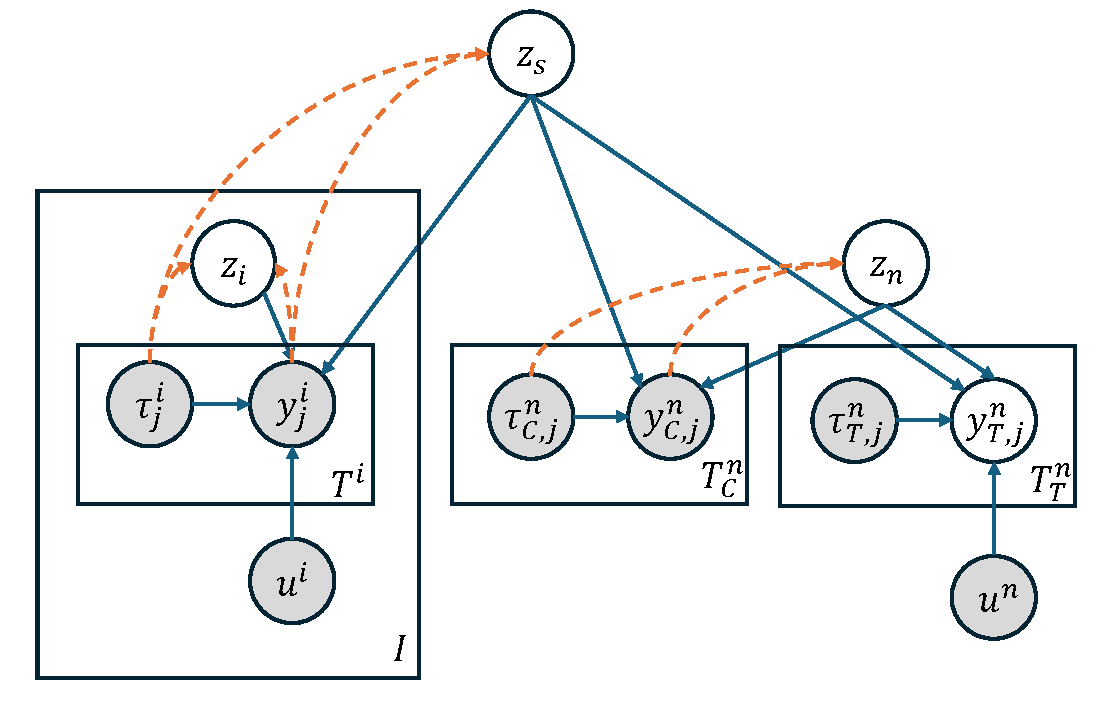
\includegraphics[width=0.42\linewidth]{figures/GraphicalModel-with-u-in-encoder.pdf}\hfill
    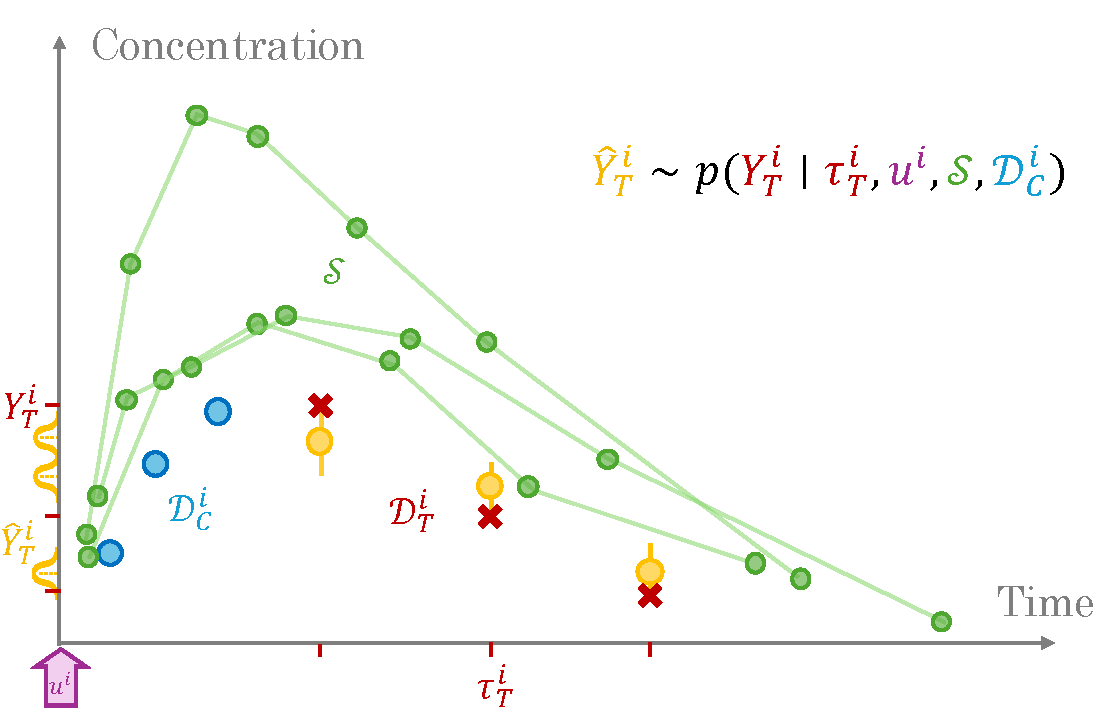
\includegraphics[width=0.42\linewidth]{figures/NotationIllustration.pdf}
    \caption{\small
    Left: AICMET separates study-level latent effects $z_s$ from individual-level effects $z_i$.
    Right: predictions combine study context $\mathcal S$, individual context $\mathcal D_C^i$,
    dosing $\mathbf u^i$, and target times $\boldsymbol\tau_T^i$.}
    \label{fig:graphical-model}
\end{figure}

\vspace{-0.4em}

\textbf{Synthetic PK prior.}
AICMET is pretrained on pharmacologically structured synthetic studies generated as

\vspace{0.25em}
\begin{equation*}
\begin{aligned}
&p(\boldsymbol{\eta},T_{\mathrm{peak}},T_{\mathrm{half}},
\boldsymbol{\theta},\boldsymbol{\mu},\boldsymbol{\tau},\mathbf X,\mathbf Y)
\\[0.35em]
&\qquad =
p(\boldsymbol{\eta})\,
p(T_{\mathrm{peak}},T_{\mathrm{half}}\mid\boldsymbol{\eta})
\prod_{i=1}^{I}
p_i^{\mathrm{init}}\,
p_i^{\mathrm{sample}}\,
p_i^{\mathrm{dyn}}\,
p_i^{\mathrm{obs}},
\\[0.75em]
&p_i^{\mathrm{dyn}}
=
\prod_{t\in\mathcal T}
p_{\mathrm{OU}}\!\left(
\boldsymbol{\theta}_i(t+\Delta t)
\mid
\boldsymbol{\theta}_i(t),\boldsymbol{\eta},\boldsymbol{\mu}_i
\right)
p_{\mathrm{ode}}\!\left(
\mathbf X^i(t+\Delta t)
\mid
\mathbf X^i(t),\boldsymbol{\theta}_i(t)
\right),
\\[0.75em]
&p_i^{\mathrm{obs}}
=
\prod_{j=1}^{T_i}
p_{\mathrm{obs}}\!\left(
y_j^i
\mid
\mathbf X^i(\tau_j^i),
\boldsymbol{\theta}_i(\tau_j^i)
\right).
\end{aligned}
\end{equation*}

\vspace{0.1em}
with
\[
p_i^{\mathrm{init}}
=
p(\boldsymbol{\theta}_i(0),\boldsymbol{\mu}_i\mid\boldsymbol{\eta})\,
p(\mathbf X^i(0)),
\qquad
p_i^{\mathrm{sample}}
=
p(\boldsymbol{\tau}^i\mid T_{\mathrm{peak}},T_{\mathrm{half}}).
\]

\vspace{-0.25em}

\begin{itemize}
    \setlength\itemsep{0.1em}
    \item $p_{\mathrm{OU}}$: stochastic time-varying PK parameters inducing realistic inter-individual variability.
    \item $p_{\mathrm{ode}}$: compartment dynamics for absorption, distribution, and elimination.
    \item $p_{\mathrm{obs}}$: noisy concentration measurements at sparse and irregular sampling times.
\end{itemize}

\vspace{0.2em}
\metricbox{Takeaway}{
Mechanistic simulations provide pharmacological inductive bias; in-context transformers amortize mixed-effects inference for zero-shot PK prediction.
}

\end{block}
\end{column}

  \begin{column}{0.325\textwidth}

\begin{block}{AICMET Model: Encoder, Decoder \& Objectives}
\justifying
\small

\subhead{Encoder--decoder model}

AICMET uses a hierarchical latent representation with Gaussian priors
$\mathbf z_s\sim\mathcal N(0,I)$ and $\mathbf z_i\sim\mathcal N(0,I)$:
the study code $\mathbf z_s$ captures population-level effects, while individual codes $\mathbf z_i$ capture subject-specific deviations. The encoder approximates
\[
q_\phi\!\left(
\mathbf z_s,\{\mathbf z_i\}_{i=1}^{I},\mathbf z_n
\mid \mathcal S^n
\right)
=
q_\phi(\mathbf z_s\mid\mathcal S^n)\,
q_\phi(\mathbf z_n\mid\mathcal D^n)
\prod_{i=1}^{I}q_\phi(\mathbf z_i\mid\mathcal D^i),
\]
and the decoder predicts concentrations through
\[
p_\theta(\mathbf Y\mid \mathbf z_s,\{\mathbf z_i,\mathbf u^i,\boldsymbol\tau^i\}_{i=1}^{I})
=
\prod_{i=1}^{I}
\prod_{j=1}^{T_i}
\mathcal N\!\left(
y_j^i
\mid
\mu_\theta(\tau_j^i,\mathbf Z_i),
\sigma_\theta^2(\tau_j^i,\mathbf Z_i)
\right),
\qquad
\mathbf Z_i=(\mathbf z_s,\mathbf z_i,\mathbf u^i).
\]

\vspace{0.2em}

\begin{figure}[t]
    \centering
    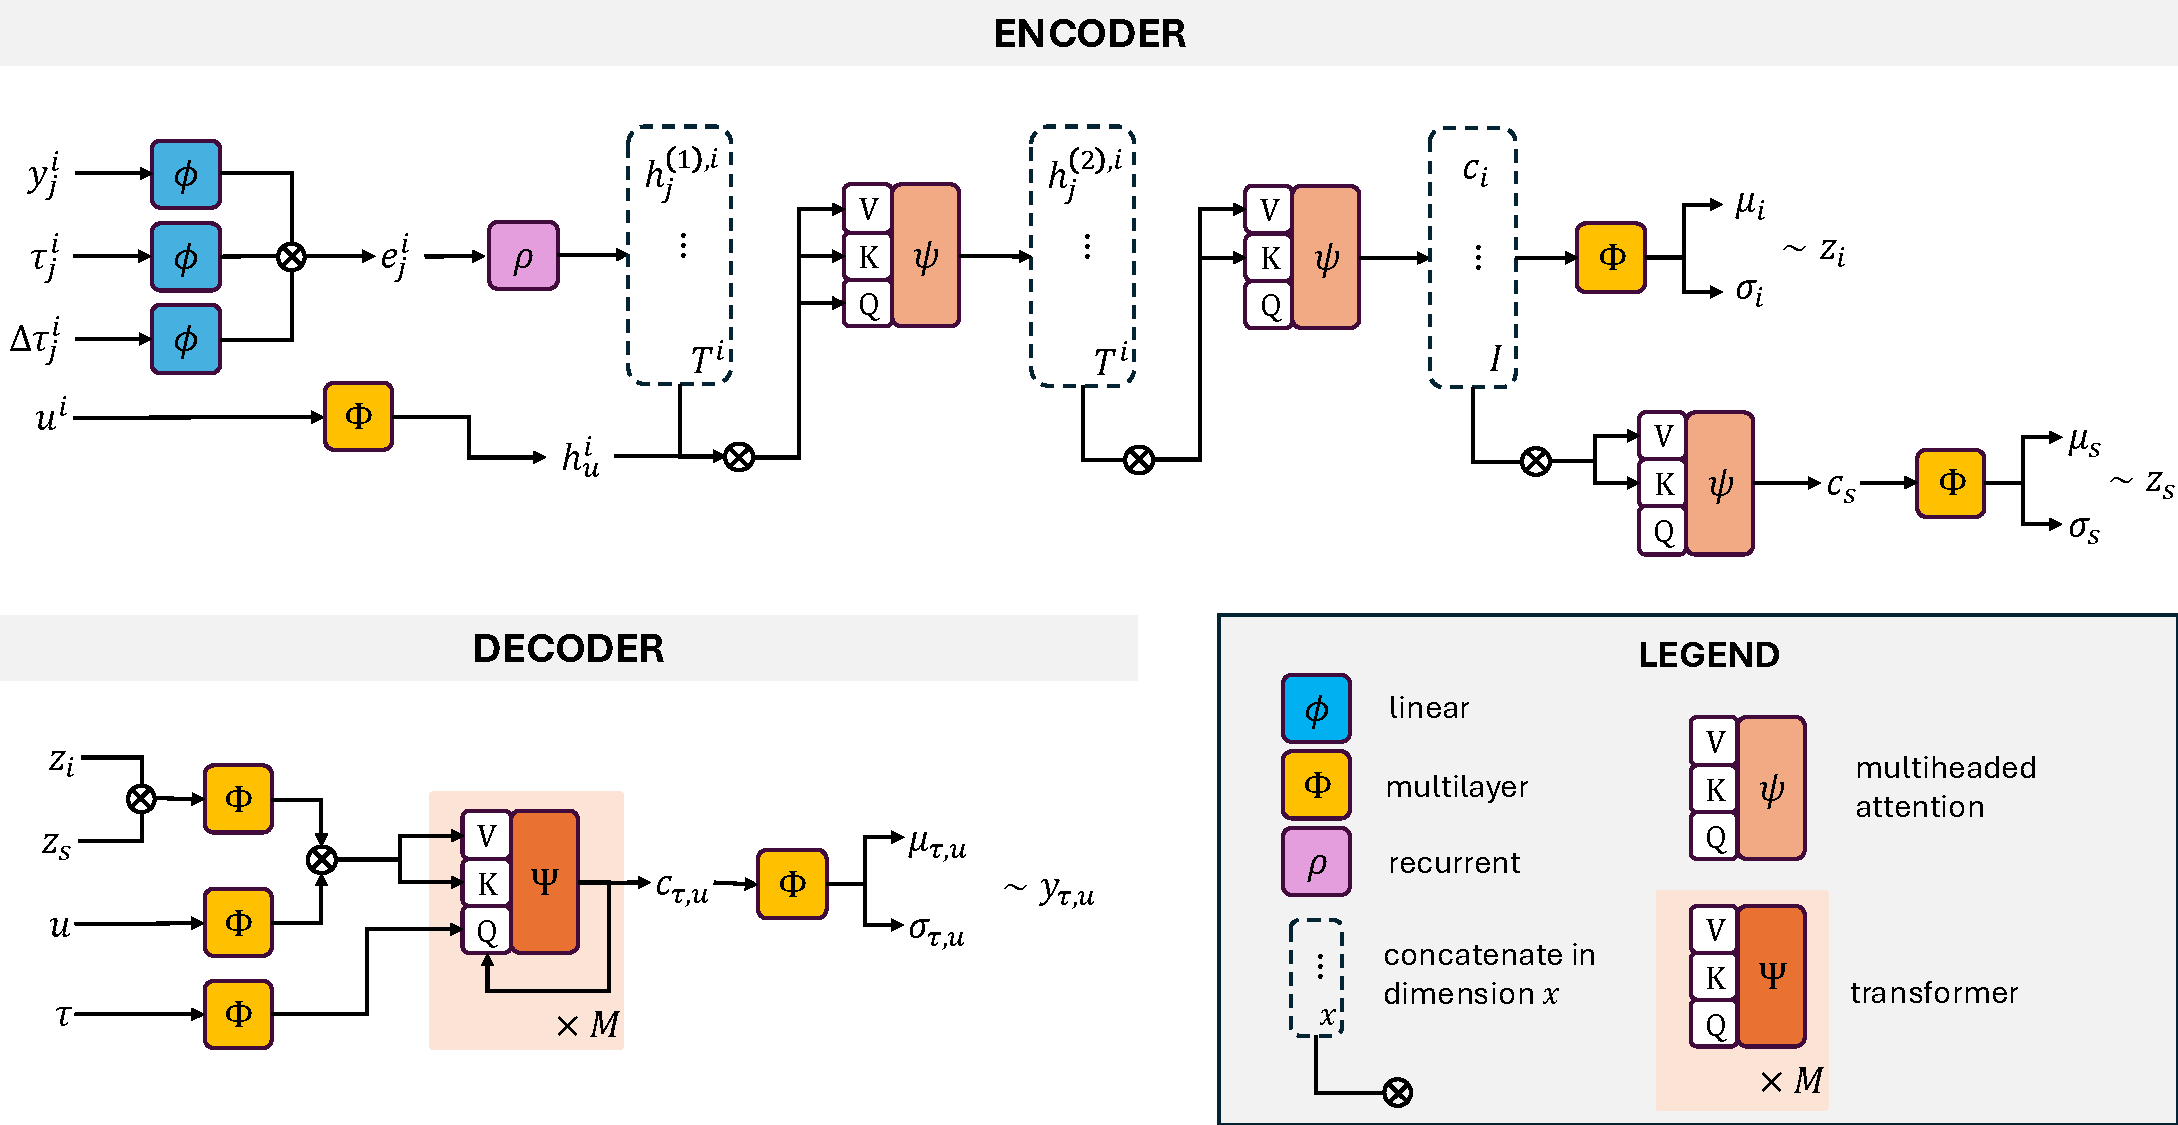
\includegraphics[width=0.75\linewidth]{figures/NetworkArchitectureSketch-V2.pdf}
    \vspace{-0.4em}
    \caption{\small
    AICMET architecture. The encoder produces dynamic representations with a recurrent backbone, and attention mechanisms summarize them at both individual and study levels. The transformer decoder embeds these representations alongside dose information and uses functional queries to evaluate the predictive distribution at any target time $\tau$.}
    \label{fig:architecture}
\end{figure}

\vspace{-0.35em}

\subhead{Training objectives}

The first objective holds out one individual and learns to predict it from the study context:
\[
\begin{aligned}
\mathcal L_{\mathrm{new}}
&=
\mathbb E_q
\left[
\log p_\theta(\mathbf Y^n
\mid \mathbf z_s,\mathbf z_n,\mathbf u^n,\boldsymbol\tau^n)
\right]
-
\mathrm{KL}\!\left[
q(\mathbf z_s\mid\mathcal S)\,\|\,p(\mathbf z_s)
\right]
\\[-0.15em]
&\quad
-
\mathrm{KL}\!\left[
q(\mathbf z_n\mid\mathcal D^n)\,\|\,p(\mathbf z_n)
\right]
-
\mathrm{KL}\!\left[
q(\mathbf z_s\mid\mathcal S^n)\,\|\,q(\mathbf z_s\mid\mathcal S)
\right].
\end{aligned}
\]

\vspace{0.2em}

The second objective trains context-to-target prediction within each individual trajectory:
\[
\begin{aligned}
\mathcal L_{\mathrm{P}}
&=
\mathbb E_{q(\mathbf z_s\mid\mathcal S)}
\left[
\sum_{i=1}^{I}
\mathbb E_{q(\mathbf z_i\mid\mathcal D^i)}
\log p_\theta(
\mathbf Y_T^i
\mid
\mathbf z_s,\mathbf z_i,\mathbf u^i,\boldsymbol\tau_T^i)
\right]
-
\sum_{i=1}^{I}
\mathrm{KL}\!\left[
q(\mathbf z_i\mid\mathcal D^i)
\,\|\, 
q(\mathbf z_i\mid\mathcal D_C^i)
\right].
\end{aligned}
\]

\vspace{0.2em}
\metricbox{Takeaway}{
AICMET amortizes mixed-effects inference: encode sparse study data into population and individual latents, then decode dose-conditioned concentration distributions at arbitrary times.
}

\end{block}

\end{column}

\begin{column}{0.345\textwidth}

    \begin{block}{Prediction: $N=20$}
    \begin{figure}[t]
    \centering

    \begin{minipage}[b]{0.30\linewidth}
        \centering
        {\small (a)}\\[-0.4em]
        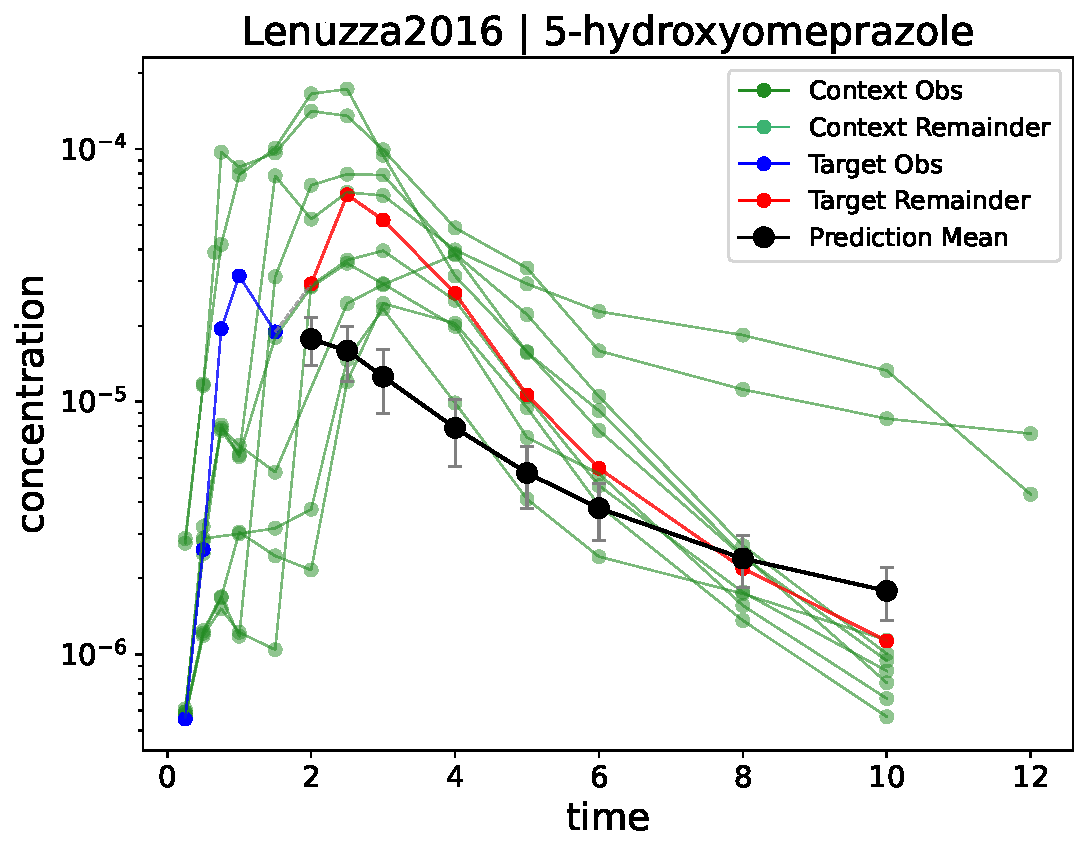
\includegraphics[width=0.88\linewidth]{figures/5_hydroxyomeprazole_prediction.pdf}
    \end{minipage}
    \hfill
    \begin{minipage}[b]{0.30\linewidth}
        \centering
        {\small (b)}\\[-0.4em]
        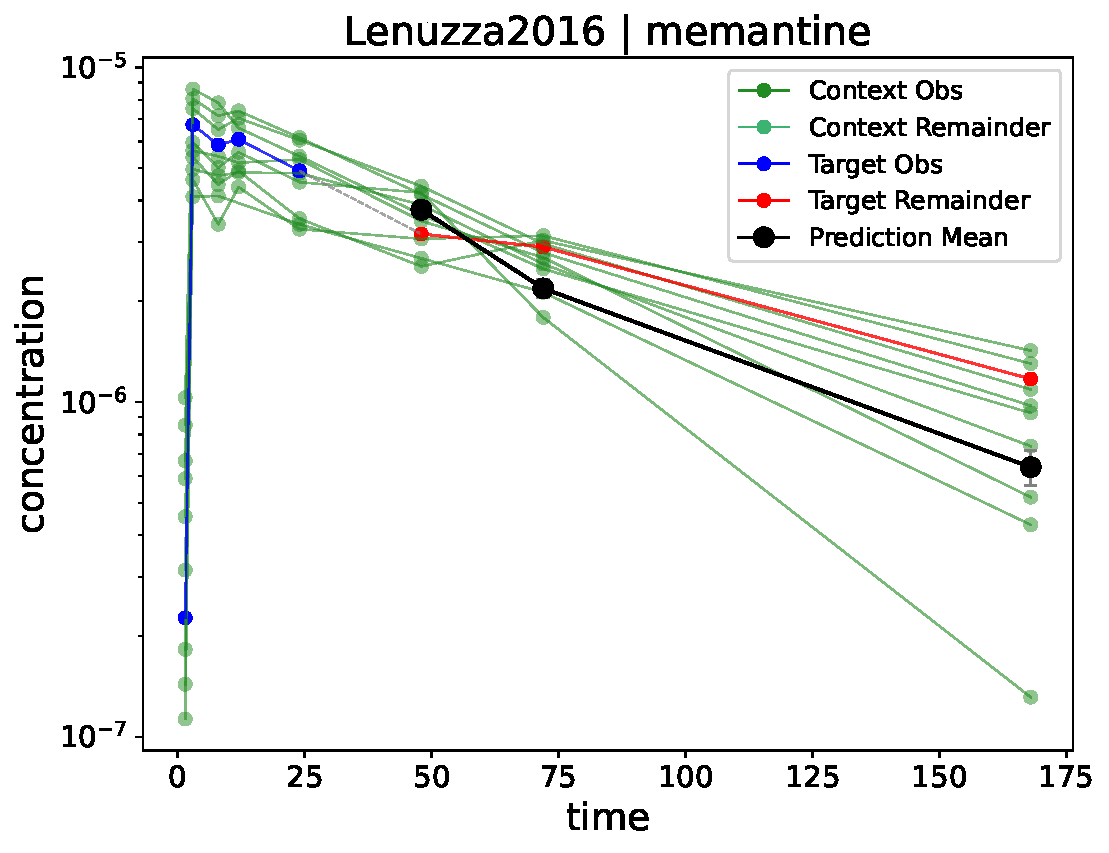
\includegraphics[width=0.88\linewidth]{figures/memantine_prediction.pdf}
    \end{minipage}
    \hfill
    \begin{minipage}[b]{0.30\linewidth}
        \centering
        {\small (c)}\\[-0.4em]
        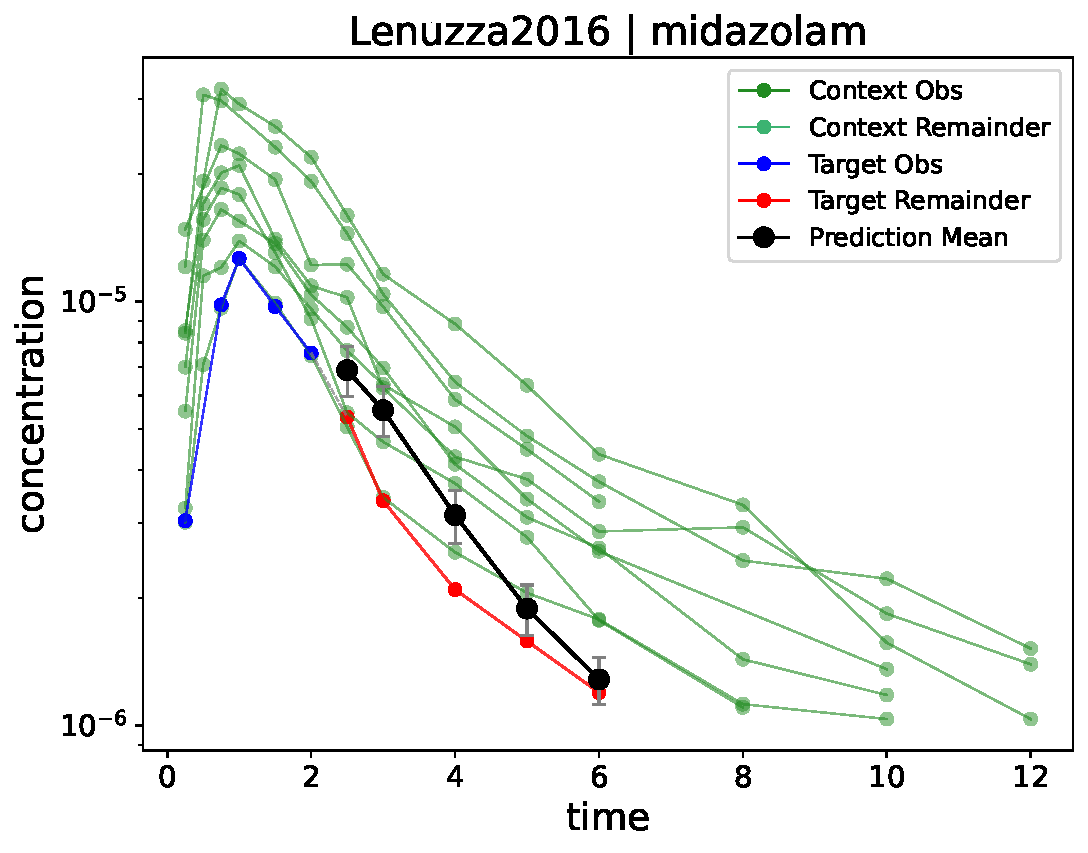
\includegraphics[width=0.88\linewidth]{figures/midazolam_prediction.pdf}
    \end{minipage}

    \vspace{-0.9em}
    \caption{\small Zero-shot  prediction curves for three compounds.}
    \label{fig:prediction_triplet}
    \end{figure}
    \end{block}


    \begin{block}{Zero-Shot Visual Predictive Checks}
    \begin{figure}[t]
    \centering

    \begin{minipage}[b]{0.46\linewidth}
        \centering
        {\small (a)}\\[-0.4em]
        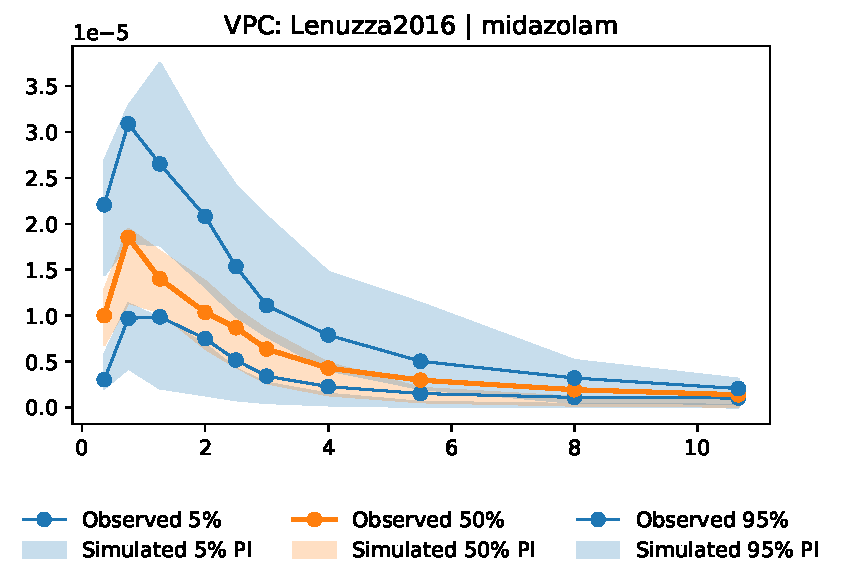
\includegraphics[width=0.88\linewidth]{figures/midazolam_vpc.pdf}
    \end{minipage}
    \hfill
    \begin{minipage}[b]{0.46\linewidth}
        \centering
        {\small (b)}\\[-0.4em]
        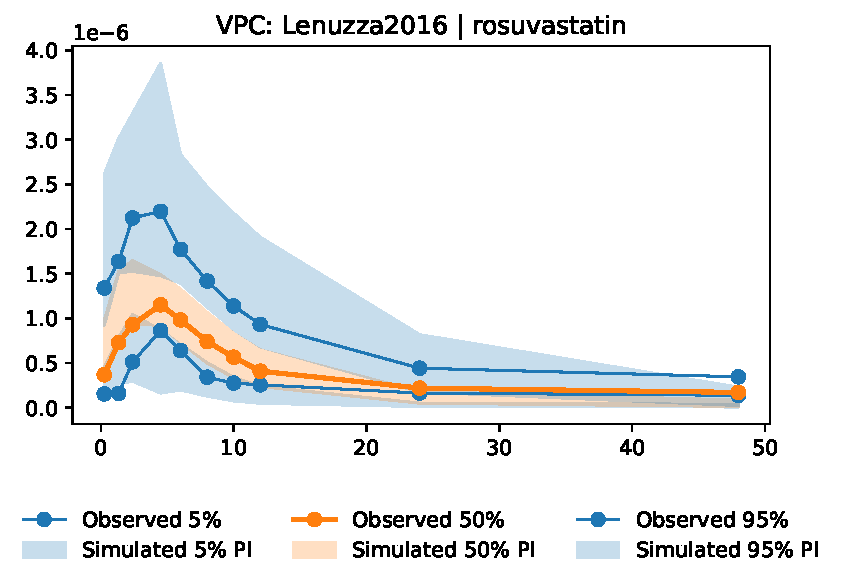
\includegraphics[width=0.88\linewidth]{figures/rosuvastatin_vpc.pdf}
    \end{minipage}

    \vspace{-0.9em}
    \caption{\small Zero-shot VPCs comparing observed summaries with simulation-based prediction intervals.}
    \label{fig:vpc_column}
    \end{figure}
    \end{block}

\begin{block}{Selected Log-RMSE Results}
  {\fontsize{14}{17}\selectfont
  \centering
  \renewcommand{\arraystretch}{1.02}
  \setlength{\tabcolsep}{4pt}
  \resizebox{0.98\linewidth}{!}{%
  \begin{tabular}{lcccc}
  \hline
  \textbf{Compound} & \textbf{NODE-PK} & \textbf{ST-PK} & \textbf{AICME-NODE} & \textbf{AICMET} \\
  \hline
  midazolam 
  & $0.352 \pm 0.224$ 
  & $0.288 \pm 0.173$ 
  & $0.548 \pm 0.209$ 
  & $\mathbf{0.264 \pm 0.151}$ \\

  repaglinide 
  & $0.693 \pm 0.290$ 
  & $0.709 \pm 0.268$ 
  & $0.562 \pm 0.204$ 
  & $\mathbf{0.339 \pm 0.311}$ \\

  theophylline 
  & $0.327 \pm 0.144$ 
  & $0.356 \pm 0.141$ 
  & $0.318 \pm 0.126$ 
  & $\mathbf{0.274 \pm 0.109}$ \\

  tolbutamide 
  & $0.578 \pm 0.263$ 
  & $0.678 \pm 0.339$ 
  & $0.854 \pm 0.316$ 
  & $\mathbf{0.517 \pm 0.254}$ \\

  dextrorphan 
  & $0.834 \pm 0.284$ 
  & $0.733 \pm 0.445$ 
  & $0.614 \pm 0.229$ 
  & $\mathbf{0.563 \pm 0.287}$ \\
  \hline
  \end{tabular}
  }
  \par}

  \vspace{0.15em}
  {\footnotesize
  AICMET obtains the lowest log-RMSE on several compounds, showing competitive zero-shot adaptation from contextual PK observations.
  }
\end{block}

\end{column}


\end{columns}

\end{frame}
\end{document}
